\chapter{Trace Encoder Output Packets} \label{packets}

The bulk of this section describes the payload of packets output from the Trace Encoder.  
The infrastructure used to transport these packets is outside the scope of this document, and
as such the manner in which packets are encapsulated for transport is not specified.
However, the following information must be provided to the encapsulator:

\begin{itemize}
  \item The packet type;
  \item The packet length, in bytes;
  \item The packet payload.
\end{itemize}

Two example transport schemes are the UltraSoC Messaging Infrastructure, and the Arm Trace Bus.
Figure~\ref{fig:packet-format} shows the encapsulation used for the UltraSoC infrastructure:
\begin{itemize}
  \item The header byte contains a 5-bit field specifying the payload length in bytes, a 2-bit
    field indicating the "flow" (destination routing indicator), and a bit to indicate whether
    an optional 16-bit timestamp is present;
  \item The index field indicates the source of the packet.  The number of bits is system dependent,
    And the initial value emitted by the trace encoder is zero (it gets adjusted as it propagates 
    through the infrastructure);
  \item An optional 2-byte timestamp;
  \item The packet payload.
\end{itemize}

\begin{figure}[h]
  \begin{center}
    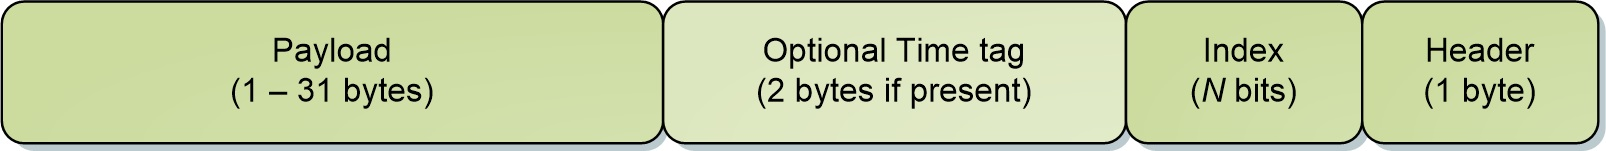
\includegraphics[height=1cm, width=9cm]{newPacket.jpg}
    \caption{Example Encapsulated Packet Format}
    \label{fig:packet-format}
  \end{center}
\end{figure}


Alternatively, for ATB, the source of the packet is indicated by the \textbf{ATID} bus field, and there is
no equivalent of "flow", so an example encapsulation might be:
\begin{itemize}
  \item A 5-bit field specifying the payload length in bytes
  \item A bit to indicate whether an optional 16-bit timestamp is present;
  \item An optional 2-byte timestamp;
  \item The packet payload.
\end{itemize}
It may be desirable for packets to start aligned to an ATB word, in which the \textbf{ATBYTES} bus field
in the last beat of a packet can be used to indicate the number of valid bytes.

The remainder of this section describes the contents of the payload
portion which should be independent of the infrastructure.  In each table, the fields are listed in
transmission order: first field in the table is transmited first, and multi-bit fields are 
transmitted LSB first.

This packet payload format is used to output encoded instruction
trace.  Three different formats are used according to the needs of the
encoding algorithm. The following tables show the format of the
payload - i.e. excluding any encapsulation.

In order to achieve best performance, actual packet lengths may be adjusted using 'sign based compression'.
At the very minimum this should be applied to the address field of format 1 and 2 packets, but ideally will 
be applied to the whole packet, regardless of format.  This technique eliminates identical bits from the most 
significant end of the packet, and adjusts the length of the packet accordingly.  A decoder receiving this 
shortened packet can reconstruct the original full-length packet by sign-extending from the most significant
received bit.  An example of how this technique is used to choose between address formats is given in 
Section~\ref{addresses}.  The same principal can be applied to the entire packet, and the length (typically 
given in bytes) adjusted accordingly.

Where the payload length given in the following tables, or after applying sign-based compression, is not a 
multiple of whole bytes in length, the payload must be sign-extended to the nearest byte boundary.

Whilst offering maximum encoding efficiency, variable length packets can present some challenges,
specifically in terms of identifying where the boundaries between packets occur either when packed
packets are written to memory, or when packets are streamed offchip via a communications channel.  Two 
potential solutions to this are as follows:

\begin{itemize}
  \item If the maximum packet payload length is 2\textsuperscript{N}-1 (for example, if N is 5, then the maximum length is
    31 bytes), and the minimum packet payload length is 1, then a sequence of at least 2\textsuperscript{N} zero 
    bytes cannot occur within a packet payload, and therefore the first non-zero byte seen after a sequence of 
    at least 2\textsuperscript{N} zero bytes must be the first byte of a packet.  This approach can be used for
    alignment in either memory or a data stream;
  \item An alternative approach suitable for packets written to memory is to divide memory into blocks of M bytes
    (e.g. 1kbyte blocks), and write packets to memory such that the first byte in every block is always the first
    byte of a packet.  This means packets cannot span block boundaries, and so zero bytes must be used to pad between 
    the end of the last message in a block and the block boundary.
\end{itemize}

\begin{table}[htp]
  \centering
  \caption{Packet Payload Format 1 - with address}
  \label{tab:te_inst0-1-addr}
  \begin{tabulary}{\textwidth}{|l|p{35mm}|p{80mm}|}
    \hline
    {\bf Field name} & {\bf Bits} & {\bf Description} \\
    \hline
    \textbf{format}	& 2	& 01 (diff-delta): includes branch map and differential address\\
    \hline
    \textbf{branches} & 5 & Number of valid bits in branch-map. The length of branch-map is determined as follows: \newline
    0:      (cannot occur for this format) \newline
    1: 	1 bit \newline
    2-9: 	9 bits \newline
    10-17: 	17 bits \newline
    18-25: 	25 bits \newline
    26-31: 	31 bits \newline
    For example if branches = 12, the branch-map is 17 bits long, and the 12 LSBs are valid. \newline
    In most cases when the branch map is full there is no need to report an address,
    and this is indicated by setting branches to 0.  The exception to this is when 
    the instruction immediately prior to the final branch causes an uninferable discontinuity.\\
    \hline
    \textbf{branch\_map} & Determined by \newline 
                 \textbf{branches} field. & 
                 An array of bits indicating whether branches are taken or not.\newline
    Bit 0 represents the oldest branch instruction executed.   For each bit: \newline
    0: branch taken \newline
    1: branch not taken \\
    \hline
    \textbf{address}	& \textit {iaddress\_width\_p - iaddress\_lsb\_p} & 
                Differential instruction address.\\
    \hline
  \end{tabulary}
\end{table}

\begin{table}[htp]
  \centering
  \caption{Packet Payload Format 1  - no address, branch map}
  \label{tab:te_inst0-1-noaddr-map}
  \begin{tabulary}{\textwidth}{|l|p{35mm}|p{80mm}|}
    \hline
    {\bf Field name} & {\bf Bits} & {\bf Description} \\
    \hline
    \textbf{format}	& 2	& 01 (diff-delta): includes branch map and differential address\\
    \hline
    \textbf{branches} & 5 & Number of valid bits in branch-map. The length of branch-map is determined as follows: \newline
    0:      31 bits, no \textbf{address} in packet \newline
    1-31: 	(cannot occur for this format) \\
    \hline
    \textbf{branch\_fmt} & 1  & Set to 0, indicating next field is \textbf{branch\_map}. \\
    \hline
    \textbf{branch\_map} & 31 & 
                 An array of bits indicating whether branches are taken or not.\newline
    Bit 0 represents the oldest branch instruction executed.   For each bit: \newline
    0: branch taken \newline
    1: branch not taken \\
    \hline
  \end{tabulary}
\end{table}

\begin{table}[htp]
  \centering
  \caption{Packet Payload Format 1 - no address, branch count}
  \label{tab:te_inst0-1-noaddr-count}
  \begin{tabulary}{\textwidth}{|l|p{35mm}|p{80mm}|}
    \hline
    {\bf Field name} & {\bf Bits} & {\bf Description} \\
    \hline
    \textbf{format}	& 2	& 01 (diff-delta): includes branch map and differential address\\
    \hline
    \textbf{branches} & 5 & Number of valid bits in branch-map. The length of branch-map is determined as follows: \newline
    0:      31 bits, no \textbf{address} in packet \newline
    31-1: 	(cannot occur for this format) \\
    \hline
    \textbf{branch\_fmt} & 1  & Set to 1, indicating next fields are \textbf{branch\_count} and \textbf{no\_mispred}. \\
    \hline
    \textbf{branch\_count} & 16 & Count of the number of correctly predicted	 branches, minus 31. \\
    \hline
    \textbf{no\_mispred} & 1 & 
                 Set to 0 if next branch failed prediction.  Set to 1 if packet is output because of an updiscon, 
                 exception or because \textbf{branch\_count} has reached 0xffff. \\
    \hline
  \end{tabulary}
\end{table}


\begin{table}[!h]
  \centering
  \caption{Packet Payload Format 2}
  \label{tab:te_inst2}
  \begin{tabulary}{\textwidth}{|l|p{35mm}|p{80mm}|}
    \hline
    {\bf Field name} & {\bf Bits} & {\bf Description} \\
    \hline
    \textbf{format}	& 2	& 10 (addr-only): differential address and no branch map\\
    \hline
    \textbf{address} & \textit {iaddress\_width\_p - iaddress\_lsb\_p} & 
              Differential instruction address.\\ 
    \hline
  \end{tabulary}
\end{table}

\begin{table}[htp]
  \centering
  \caption{Packet Payload Format 3, subformat 0}
  \label{tab:te_inst3}
  \begin{tabulary}{\textwidth}{|l|p{35mm}|p{80mm}|}
    \hline
    {\bf Field name} & {\bf Bits} & {\bf Description} \\
    \hline
    \textbf{format} & 2 & 11 (sync): synchronisation\\
    \hline
    \textbf{subformat} & 2 & 00 (start): Start of tracing, or resync \\
    \hline
    \textbf{context} &  \textit {context\_width\_p}, 
               or 0 if \textit {nocontext\_p} is 1 & 
               The instruction context \\
    \hline
    \textbf{privilege} & \textit {privilege\_width\_p} & 
                The current privilege level \\
    \hline
    \textbf{branch} & 1 & If the address points to a branch instruction, set to 1 if the branch was not taken. 
    Has no meaning if this instruction is not a branch. \\
    \hline
    \textbf{address} & \textit {iaddress\_width\_p - iaddress\_lsb\_p} & 
              Full instruction address.  Address alignment is determined by \textit {iaddress\_lsb\_p} Address must be left shifted in order to recreate original byte address \\
    \hline
  \end{tabulary}
\end{table}

\begin{table}[htp]
  \centering
  \caption{Packet Payload Format 3, subformat 1}
  \label{tab:te_inst3}
  \begin{tabulary}{\textwidth}{|l|p{35mm}|p{80mm}|}
    \hline
    {\bf Field name} & {\bf Bits} & {\bf Description} \\
    \hline
    \textbf{format} & 2 & 11 (sync): synchronisation\\
    \hline
    \textbf{subformat} & 2 & 01 (exception): Exception cause and trap handler address\\
    \hline
    \textbf{context} &  \textit {context\_width\_p}, 
               or 0 if \textit {nocontext\_p} is 1 & 
               The instruction context \\
    \hline
    \textbf{privilege} & \textit {privilege\_width\_p} & 
                The current privilege level \\
    \hline
    \textbf{branch} & 1 & If the address points to a branch instruction, set to 1 if the branch was not taken. 
    Has no meaning if this instruction is not a branch. \\
    \hline
    \textbf{address} & \textit {iaddress\_width\_p - iaddress\_lsb\_p} & 
              Full instruction address.  Address alignment is determined by \textit {iaddress\_lsb\_p} Address must be left shifted in order to recreate original byte address \\
    \hline
    \textbf{ecause} & \textit {ecause\_width\_p} & 
             Exception cause \\
    \hline
    \textbf{interrupt} & 1 & 
                Interrupt \\
    \hline
    \textbf{tval} & \textit {iaddress\_width\_p}, 
           or 0 if \textit {notval\_p} is 1 & 
           Trap value \\
    \hline
  \end{tabulary}
\end{table}

\begin{table}[htp]
  \centering
  \caption{Packet Payload Format 3, subformat 2}
  \label{tab:te_inst3}
  \begin{tabulary}{\textwidth}{|l|p{35mm}|p{80mm}|}
    \hline
    {\bf Field name} & {\bf Bits} & {\bf Description} \\
    \hline
    \textbf{format} & 2 & 11 (sync): synchronisation\\
    \hline
    \textbf{subformat}  & 2 & 10 (context): Context change \\
    \hline
    \textbf{context} &  \textit {context\_width\_p} & The instruction context \\
      \hline
  \end{tabulary}
\end{table}

\begin{table}[htp]
  \centering
  \caption{Packet Payload Format 3, subformat 3}
  \label{tab:te_inst3}
  \begin{tabulary}{\textwidth}{|l|p{35mm}|p{80mm}|}
    \hline
     {\bf Field name} & {\bf Bits} & {\bf Description} \\
     \hline
     \textbf{format} & 2 & 11 (sync): synchronisation\\
     \hline
     \textbf{subformat}  & 2 & 11 (support): Supporting information for the decoder \\
     \hline
     \textbf{enable} & 1 & Indicates if encoder is enabled\\
     \hline
     \textbf{encoder\_mode} & N & Identifies trace algorithm\newline
       Details implementation dependent.  Currently Branch trace is the only mode defined.\\
     \hline
     \textbf{qual\_status} & 2 & Indicates qualification status\newline
       00 (no\_change): No change to filter qualification \newline
       01 (ended\_rep): Qualification ended, preceding \textbf{te\_inst} sent explicitly to indicate last qualification instruction\newline
       10: (packet\_lost): One or more packets lost.\newline
       11 : (ended\_ntr): Qualification ended, no unreported instructions (so preceeding \textbf{te\_inst} would have been sent anyway, even if it wasn't the last qualified instruction)\\
     \hline
     \textbf{options} & N & Values of all run-time configuration bits\newline
       Number of bits and definitions implementation dependent.  Examples might be\newline
       - 'implicit return' Don't report function return addresses \newline
       - 'implicit exception' Exclude address from format 3, sub-format 1 \textit{te\_inst} packets if trap vector can be determined from \textit{ecause field}\newline
       - 'branch prediction' Branch predictor enabled\newline
       - 'full address' Always output full addresses (SW debug option)\\
       \hline
  \end{tabulary}
\end{table}
